\chapter{Результаты}
Результаты попарной классификации для пар классов (AD, NC), (AD, LMCI), (LMCI, EMCI), (EMCI, NC), полученные на базовых алгоритмах, представлены в таблице ниже:
\begin{table}[h]
\centering
\begin{tabular}{lll}
\rowcolor[HTML]{EFEFEF} 
\hline
Пара классов & SVM + L2 расстояние & SVM + SPD регуляризация \\
\hline
(AD, NC)     & 77.2 $\pm$ 0.99     & 80 $\pm$ 0.54       \\
(AD, LMCI)   & 65.5 $\pm$ 1.6      & 68.8 $\pm$ 0.81     \\
(LMCI, EMCI) & 44.7 $\pm$ 2.9      & 47.8 $\pm$ 2.4      \\
(EMCI, NC)   & 50.4 $\pm$ 1.8      & 53.9 $\pm$ 1.6     
\end{tabular}
\caption{Результаты классификации базовых алгоритмов, метрика качества – ROC AUC \eqref{roc-auc}}
\end{table}

На рисунке ниже представлена зависимость качества классификации предложенных в работе методов в зависимости от параметра $k$ в формуле расстояния на СППО многообразии \eqref{spsd-distance}
\begin{figure}[h!]
\centering
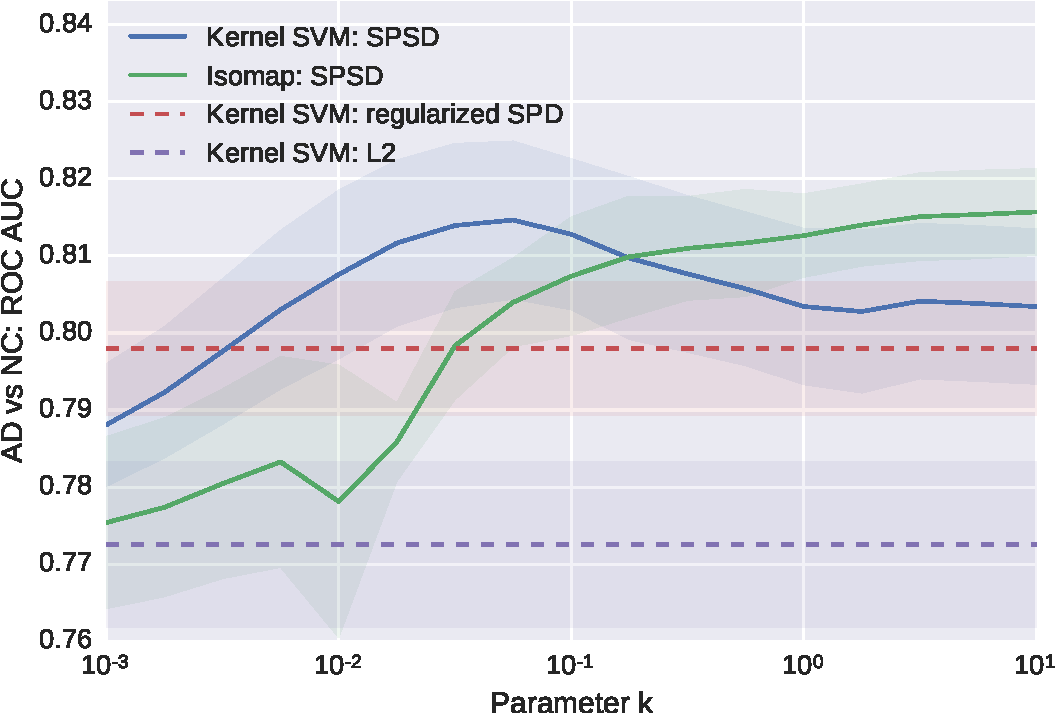
\includegraphics[width=0.8\textwidth]{img/k_dep.pdf}\label{fig:clf_quality}
\caption{Качество классификации как функция от параметра $k$ в \eqref{spsd-distance}. Четыре линиис соответствуют средним значениям площади под ROC-кривой, оцененной с помощью 10-фолдной групповой кросс-валидации. Прозрачные области соответствуют среднеквадратичному отклонению}
\end{figure}

\newpage Подход с использованием снижения размерности СППО матриц изначально был применен для проекции данных на двумерное пространство, чтобы получить возможность визуально оценить распределение данных. На рисунке ниже представлена проекция всех данных классов AD и NC на двумерную плоскость. Как можно увидеть, даже такое представлене данных достаточно наглядно.

\begin{figure}[h!]
\centering
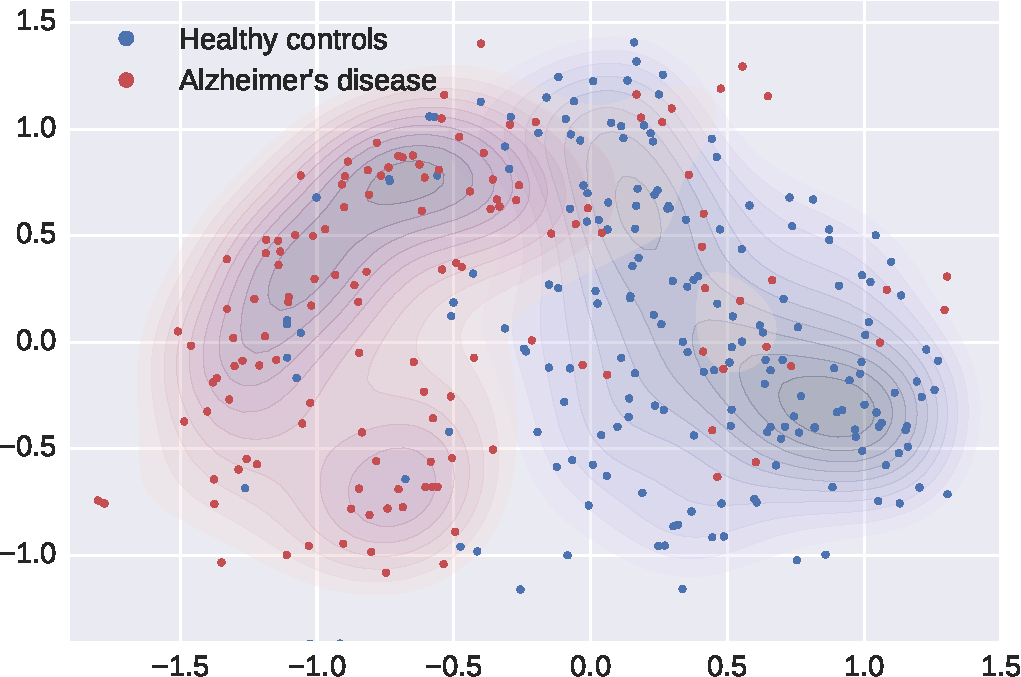
\includegraphics[width=0.8\textwidth]{img/dr.pdf}\label{fig:dr}
\caption{Структурные коннектомы для всех представителей классов AD и NC, спроецированные на двумерное пространство. Синий и красный цвета обозначают NC и AD группы соответственно. Точки соответствуют графам, прозрачные области отображают оценку плотности ядер для каждой группы}
\end{figure}

Следующая таблица содержит сравнительные результаты классификации всех четырех алгоритмов, рассматривавшихся в работе

\begin{table}[h!]
\centering
\begin{tabular}{lllll}
\hline
\rowcolor[HTML]{EFEFEF} 
Пара классов & SVM + L2 & SVM + SPD & Isomap $\delta_{spsd}$ & SVM + $\delta_{spsd}$ \\
\hline
(AD, NC)     & 77.2 $\pm$ 0.99     & 80 $\pm$ 0.54                           & \cellcolor[HTML]{E1FFCF}81.6 $\pm$ 0.6           & \cellcolor[HTML]{E1FFCF}81.6 $\pm$ 0.7                        \\
(AD, LMCI)   & 65.5 $\pm$ 1.6      & \cellcolor[HTML]{E1FFCF}68.8 $\pm$ 0.81 & 67.8 $\pm$ 0.6                                   & 68.6 $\pm$ 1.4                                                \\
(LMCI, EMCI) & 44.7 $\pm$ 2.9      & \cellcolor[HTML]{E1FFCF}47.8 $\pm$ 2.4  & 34.1 $\pm$ 0.59                                  & 44.1 $\pm$ 2.2                                                \\
(EMCI, NC)   & 50.4 $\pm$ 1.8      & 53.9 $\pm$ 1.6                          & 53.8 $\pm$ 0.12                                  & \cellcolor[HTML]{E1FFCF}{\color[HTML]{000000} 57.1 $\pm$ 1.5}
\end{tabular}
\caption{Сравнительные результаты классификации всех четырех алгоритмов, рассматривавшихся в работе. Цветом выделены лучшие результаты для каждой пары классов. Метрика качества – ROC AUC \eqref{roc-auc}}
\end{table}
\newpage
\indent Из таблицы можно увидеть, что предложенные методы показали себя лучше базовых в задаче классификации пары классов AD vs NC. \\
\indent Более того, метод, основанный на вычислении ядра для SVM c помощью расстояния на многообразии СППО матриц дал значительно лучшие результаты в задаче различения здоровых пациентов и пациентов с ранними когнитивными нарушениями. Это является важным результатом, поскольку задача ранней диагностики развития нейродегенеративных заболеваний крайне важна.